\documentclass[12pt]{article}
\usepackage[a4paper,margin=1in]{geometry}
\usepackage{amsmath,amssymb}
\usepackage{graphicx}
\usepackage{siunitx}
\sisetup{per-mode=symbol}
\usepackage{gvv}

\title{Matrix 3.2.31}
\author{ai25btech11015 -- M Sai Rithik}
\date{}

\begin{document}
\maketitle

\section*{Question (3.2.31)}
A triangle \(ABC\) can be constructed in which\[
\angle B = 60^\circ,\qquad \angle C = 45^\circ,
\] and
\[
AB + BC + AC = 12\ \text{cm}.
\]



\section*{Solution}

Side \(a=BC,\; b=CA,\; c=AB\), and angles \(A,B,C\) opposite to \(a,b,c\) respectively.
Given \(B=60^\circ,\; C=45^\circ\).

The three linear equations in the unknowns \(a,b,c\) are
\begin{align}
a + b + c &= 12, \label{eq:sum}\\
-\,a + (\cos C)\,b + (\cos B)\,c &= 0, \label{eq:xcomp}\\
0\cdot a + (\sin C)\,b - (\sin B)\,c &= 0. \label{eq:ycomp}
\end{align}

Write the augmented matrix corresponding to \eqref{eq:sum}--\eqref{eq:ycomp}:
\begin{equation}
\left[\;
\begin{array}{ccc|c}
1 & 1 & 1 & 12 \\[4pt]
-1 & \dfrac{\sqrt{2}}{2} & \dfrac{1}{2} & 0 \\[6pt]
0 & \dfrac{\sqrt{2}}{2} & -\dfrac{\sqrt{3}}{2} & 0
\end{array}
\;\right].
\label{eq:aug}
\end{equation}

Perform RREF on the augmented matrix \eqref{eq:aug}. One convenient path is:

\begin{enumerate}
\item Add row 2 to row 1 (to eliminate the \(-1\) in row 2):
\[
R_1 \gets R_1 + R_2:
\quad
\left[\;
\begin{array}{ccc|c}
0 & 1+\dfrac{\sqrt{2}}{2} & 1+\dfrac{1}{2} & 12 \\[6pt]
-1 & \dfrac{\sqrt{2}}{2} & \dfrac{1}{2} & 0 \\[6pt]
0 & \dfrac{\sqrt{2}}{2} & -\dfrac{\sqrt{3}}{2} & 0
\end{array}
\;\right].
\]

\item On Solving with RREF we get 
\begin{equation}
a = c\cdot\frac{\sqrt{3}+1}{2}, \qquad
b = c\cdot\frac{\sqrt{6}}{2},
\label{eq:relations}
\end{equation}
and from the sum \(a+b+c=12\) we get
\begin{equation}
c\left(\frac{\sqrt{3}+1}{2}+\frac{\sqrt{6}}{2}+1\right) = 12.
\label{eq:csolve}
\end{equation}

Solving \eqref{eq:csolve} for \(c\) gives
\begin{equation}
c \;=\; \frac{24}{\sqrt{3}+\sqrt{6}+3}.
\label{eq:cvalue}
\end{equation}

Substituting back, we obtain
\begin{align}
b &= \frac{\sqrt{6}}{2}\;c \;=\; \frac{12\sqrt{6}}{\sqrt{3}+\sqrt{6}+3},
\label{eq:bvalue}\\[6pt]
a &= \frac{\sqrt{3}+1}{2}\;c \;=\; \frac{12(\sqrt{3}+1)}{\sqrt{3}+\sqrt{6}+3}.
\label{eq:avalue}
\end{align}

Numerically (for quick checking):
\begin{equation}
a \approx 4.565,\quad b \approx 4.093,\quad c \approx 3.342,
\label{eq:numeric}
\end{equation}
which indeed satisfy \(a+b+c=12\).

\section*{Plot}
Place \(B=(0,0)\) and \(C=(a,0)\) and A = (c\cos B,\; c\sin B) 

\begin{figure}[h!]
    \centering
    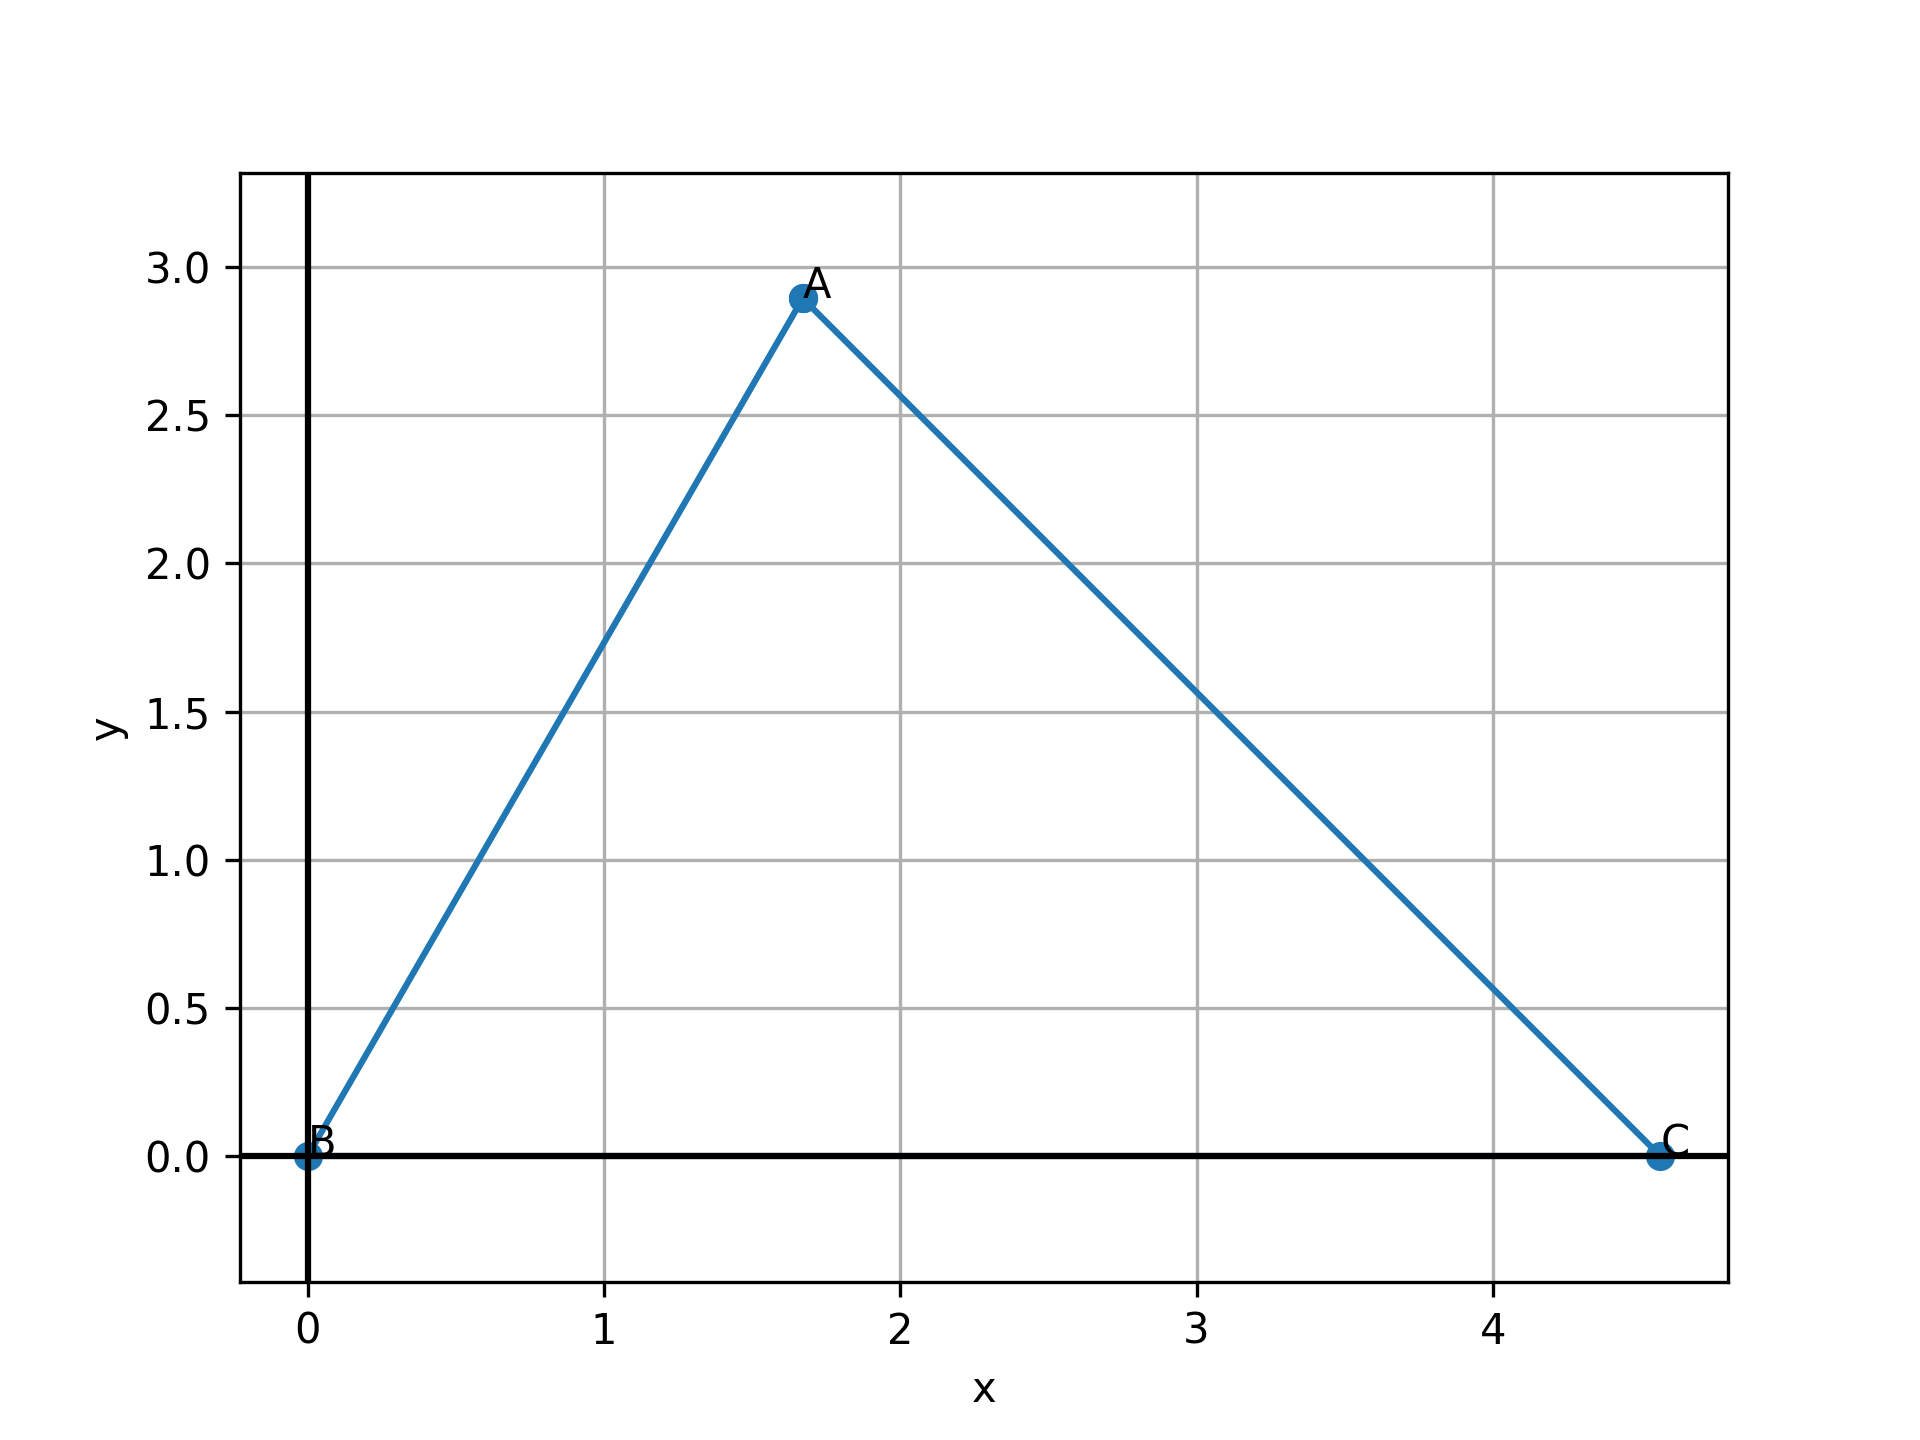
\includegraphics[width=0.65\linewidth]{figs/fig.png}
    \caption{Triangle formed by points $A$, $B$, and $C$.}
\end{figure}

\end{document}
